% !TEX encoding = UTF-8
% !TEX TS-program = pdflatex
% !TEX root = ../tesi.tex

%**************************************************************
\chapter{Verifica e validazione}
\label{cap:verifica-validazione}
%**************************************************************
\intro{In questo capitolo viene approfondito il periodo di verifica e test, durante il quale sono emerse alcune difficoltà che hanno richiesto un tempo maggiore del previsto per la risoluzione. Viene qui presentata la modalità di risoluzione di queste difficoltà, unita ai risultati ottenuti durante i test e i dati emersi dalle analisi dei risultati.}
%**************************************************************
\section{Generazione degli input}
Una volta accertato che il comportamento della \emph{\gls{bus-logic}}\glsfirstoccur\ del software prodotto fosse corretto su piccoli input di prova, si è presentato il problema di testare l'applicazione su istanze di input più grandi e con più variabili. Da piano di lavoro, il tempo previsto per verifica, testing e analisi dei risultati era stabilito di 20 ore; tuttavia, è stato da subito chiaro che il processo di verifica sarebbe stato più complicato del previsto.\\
Per eseguire test significativi in serie, era infatti necessario poter produrre automaticamente degli input su cui il software potesse elaborare per produrre schedule: è stata quindi estesa la classe \texttt{Excel} per poter andare a modificare in scrittura i fogli xls di input. In un primo momento, si è provato a generare degli input randomici, ma tale soluzione si è rivelata problematica per due motivi: in primo luogo, gli input randomici non producevano praticamente mai delle soluzioni ammissibili in quanto spesso ci si trovava con un sbilanciamento postazioni/lavoratori; in secondo luogo, anche quando veniva (raramente) prodotta una soluzione ammissibile, tale soluzione non poteva essere rappresentativa di un buono scheduling in quanto non era sensata. Il problema principale da risolvere è quindi diventato \textit{come} generare degli input il più possibile vicini alla realtà che potessero produrre degli schedule da analizzare.\\
Il problema è stato esposto al tutor aziendale, che ha approvato la modifica al piano di lavoro assegnando più ore alla verifica e al testing, tagliando su attività per il raggiungimento di requisiti desiderabili e opzionali, ritenendo più importante poter testare il software in maniera corretta e approfondita. \\
\\
Secondo le informazioni fornite dal casinò, gli input per essere realistici dovevano:
\begin{itemize}
    \item comprendere circa 30 postazioni aperte contemporaneamente, per un totale di 40 lavoratori attivi. Il totale dei lavori, per garantire quindi uno schedule fair e rispettoso delle pause e dei vincoli previsti, doveva ammontare a circa il 33\%\ in più rispetto al numero di postazioni.
    \item di tutte le postazioni aperte, alla maggior parte viene assegnato un livello basso e giochi comunemente conosciuti dai lavoratori, mentre le postazioni che richiedono un livello alto o giochi poco conosciuti sono meno.
    \item il livello dei lavoratori dipende dal tempo passato all'interno del casinò e dalle loro abilità, di conseguenze la maggior parte dei lavoratori è di livello intermedio, mentre sono pochi quelli di livello molto alto e molto basso.
    \item i giochi conosciuti dai lavoratori dipende dal loro livello: più un dealer è di livello alto, più giochi conosce; per quanto riguarda inspector e dealer-inspector, essi conoscono praticamente tutti i giochi.
\end{itemize}
Sulle basi di queste informazioni, è stato possibile produrre un modello probabilistico che descrivesse una situazione reale e progettare una nuova classe, \texttt{Test}, che generasse automaticamente ad ogni \textit{run} dell'algoritmo un set di input secondo il modello definito.

\subsection{Modello probabilistico}

Tutti i grafici presenti in questa sezione sono stati prodotti sul sito \textit{Wolphram Alpha} \cite{site:wolfram}.
    \paragraph{Numero di postazioni} Ipotizzando che il numero di postazioni aperte contemporaneamente sia circa 30, genero il numero di postazioni tramite una distribuzione normale $\mathcal{N}(\mu;\sigma \ap{2})$ con:
    \begin{itemize}
        \item tavoli: $\mu = 20$, $\sigma \ap{2} = \frac{\mu}{5}$
        \item pit: $\frac{tavoli}{3}$
    \end{itemize}
\noindent
    La \hyperref[fig61]{Figura 6.1} presenta i grafici per le distribuzioni del numero di postazioni.
    \begin{figure}[!htb]
        \label{fig61}
    \begin{widepage}
    \centering
    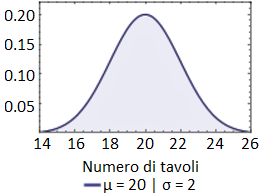
\includegraphics[width=.49\textwidth]{../immagini/gauss_tavoli_w.png}\hfil
    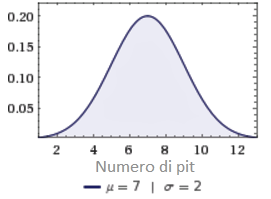
\includegraphics[width=.49\textwidth]{../immagini/gauss_pit_w.png}
    \caption{Distribuzioni normali per il numero di postazioni}
    \end{widepage}
    \end{figure}
\clearpage
    \paragraph{Costruzione delle postazioni} Ipotizzando che le postazioni che richiedono un livello alto sono poche e viceversa, genero i livelli delle postazioni L\ped{t} con una distribuzione discreta uniforme $\mathcal{U}(\mathcal{S})$ dove \[\mathcal{S} = \{ \alpha + i \, \beta \text{ t.c. } i \in \{0,2,...,n\} \} \] ovvero i cui elementi sono i progressione aritmetica con $\alpha = 1$, $\beta = 1$ e:
    \begin{itemize}
        \item per i tavoli (8 livelli): $n = 7$
        \item per i pit (3 livelli): $n = 2$
    \end{itemize}
\noindent
    La \hyperref[fig62]{Figura 6.2} presenta i grafici per le distribuzioni dei livelli delle postazioni.
    \begin{figure}[!htb]
        \label{fig62}
        \begin{widepage}
            \centering
            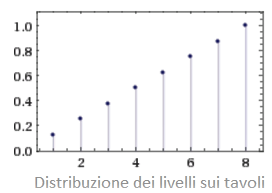
\includegraphics[width=.49\textwidth]{../immagini/discr_livelli_tavoli.png}\hfil
            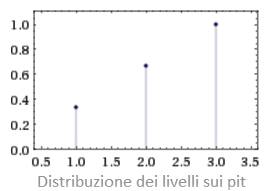
\includegraphics[width=.49\textwidth]{../immagini/discr_livelli_pit.png}
            \caption{Distribuzione discreta uniforme per i livelli delle postazioni}
        \end{widepage}
    \end{figure}
    \FloatBarrier
    \noindent
    Inoltre viene generato il gioco richiesto ad una certa postazione in modo che la frequenza del gioco base (//) sia doppia rispetto a quella di altri giochi (BJ e PG).\\
    Ad ogni postazione è richiesto un solo gioco.\\
    La \hyperref[fig63]{Figura 6.3} presenta il grafico delle frequenza di estrazione dei giochi.
    \begin{figure}[!htb]
        \label{fig63}
        \begin{widepage}
            \centering
            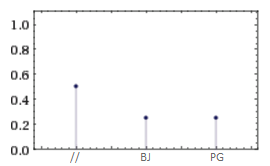
\includegraphics[width=.49\textwidth]{../immagini/distr_giochi_tavoli.png}
            \caption{Frequenza di estrazione dei giochi per ogni postazione}
        \end{widepage}
    \end{figure}%
    \clearpage
    \paragraph{Numero di lavoratori} Ipotizzando che il numero di lavoratori attivi contemporaneamente sia di circa il 33\% in più rispetto al numero di postazioni, genero il numero di lavoratori tramite una distribuzione normale $\mathcal{N}(\mu;\sigma \ap{2})$ con:
    \begin{itemize}
        \item dealer: $\mu = 1.6 \, tavoli$, $\sigma \ap{2} = \frac{tavoli}{5}$
        \item inspector: $\mu = 1.6 \, pit$, $\sigma \ap{2} = \frac{pit}{5}$
    \end{itemize}
\noindent
La \hyperref[fig64]{Figura 6.4} presenta i grafici per le distribuzioni del numero dei lavoratori.
    \begin{figure}[!htb]
        \label{fig64}
        \begin{widepage}
        \centering
        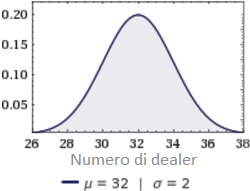
\includegraphics[width=.49\textwidth]{../immagini/gauss_dealer_w.png}\hfil
        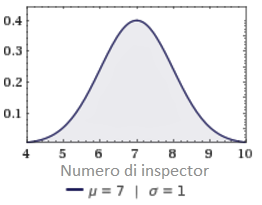
\includegraphics[width=.49\textwidth]{../immagini/gauss_inspector_w.png}
        \caption{Distribuzioni normali per il numero di lavoratori}
        \end{widepage}
    \end{figure}
    \FloatBarrier
    \noindent
    Da notare che il valor medio $\mu$ è stato fissato al 60\% in più rispetto al numero di postazioni, sarà poi compito dell'algoritmo andare ad ottimizzare il numero di lavoratori richiesti per riempire lo scheduling. \\
    \\
    Per quanto riguarda il numero di dealer-inspector, esso viene fissato a \[(tavoli + pit) \, 1.6 - dealer - inspector\] per far sì che il numero di lavoratori attivi sia sempre esattamente il 60\% in più rispetto al numero di postazioni.
    \clearpage
    \paragraph{Costruzione dei dati sui lavoratori} Ipotizzando che il livello dei lavoratori dipenda solo dal tempo che hanno passato all'interno del casinò, generiamo i livelli dei lavoratori L\ped{w} tramite una distribuzione normale $\mathcal{N}(\mu;\sigma \ap{2})$ con:
    \begin{itemize}
        \item dealer: $\mu = 4.5$, $\sigma \ap{2} = \frac{\mu}{3.5}$
        \item inspector: $\mu = 2$, $\sigma \ap{2} = \frac{\mu}{1}$
    \end{itemize}
\noindent
La \hyperref[fig65]{Figura 6.5} presenta i grafici per le distribuzioni dei livelli dei lavoratori.
     \begin{figure}[!htb]
         \label{fig65}
         \begin{widepage}
             \centering
             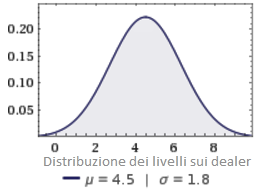
\includegraphics[width=.49\textwidth]{../immagini/livelli_dealer.png}\hfil
             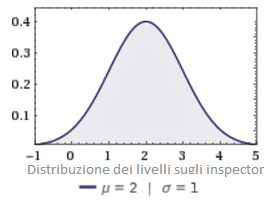
\includegraphics[width=.49\textwidth]{../immagini/livelli_insp.png}
             \caption{Distribuzioni normali per i livelli dei lavoratori}
         \end{widepage}
     \end{figure}
     \FloatBarrier
     \noindent
     Ipotizzando che la probabilità che un lavoratore conosca un gioco sia direttamente proporzionale al suo livello (più un lavoratore ha livello alto, più giochi conosce; tutti conoscono i giochi base //), generiamo i giochi che ogni lavoratore conosce con una distribuzione di Bernoulli $\mathcal{B}e(p)$ dove $p = 1 - \frac{livello}{10}$.\\
     La \hyperref[fig66]{Figura 6.6} presenta i grafici per le distribuzioni dei giochi sui lavoratori.
     \begin{figure}[!htb]
         \label{fig66}
         \begin{widepage}
             \centering
             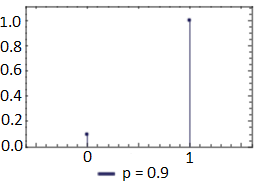
\includegraphics[width=.49\textwidth]{../immagini/livello_1.png}\hfil
             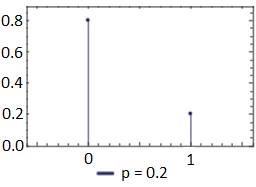
\includegraphics[width=.49\textwidth]{../immagini/livello_8.png}
             \caption{Probabilità che due lavoratori di livelli 1 (a sinistra) e 8 (a destra) conoscano un gioco (1) o meno (0)}
         \end{widepage}
     \end{figure}
 \clearpage
%**************************************************************
\section{Testing}
\subsection{Costruzione dei test}
Per eseguire i test in serie, è stato prodotto uno script Python che esegue trenta volta il programma. Ogni esecuzione genera una nuova istanza di input, costruisce gli oggetti, esegue l'algoritmo greedy producendo una soluzione e poi procede con l'ottimizzare il numero di lavoratori necessari al riempimento dello schedule.\\ Lo script Python tiene traccia, per ogni esecuzione, del tempo impiegato e di tutti gli input e output per poter poi elaborare i dati creando tre tipi di grafici:
\begin{itemize}
    \item Executions;
    \item Tests;
    \item Exec n.
\end{itemize}
\noindent
Le tre tipologie vengono presentate nei prossimi paragrafi.

    \paragraph{Grafico ``Executions''} Grafico che mette in relazione il tempo di esecuzione con la grandezza iniziale dell’input (numero tavoli, numero di lavoratori) e di quanto, tramite le iterazioni miglioranti eseguite dal software, si riesce a ridurre il numero di lavoratori. Viene messa in evidenza la media di tutti i valori.\\
    \\
    Ad esempio, la \hyperref[fig67]{Figura 6.7} presenta il grafico ``Executions'' prodotto su trenta esecuzioni dell’algoritmo.\\ Il tempo di esecuzione medio è 5.387s, il numero medio di postazioni è 27.5, il numero medio lavoratori all’inizio è di circa 46 (+68.3\% rispetto al numero di postazioni) mentre, dopo le iterazioni miglioranti, il numero medio di lavoratori è di circa 37 (+35.5\% rispetto al numero di tavoli, valore che ha un riscontro nel numero effettivo di lavoratori nel casinò di Londra).
    
    \begin{sidewaysfigure}
        \centering
        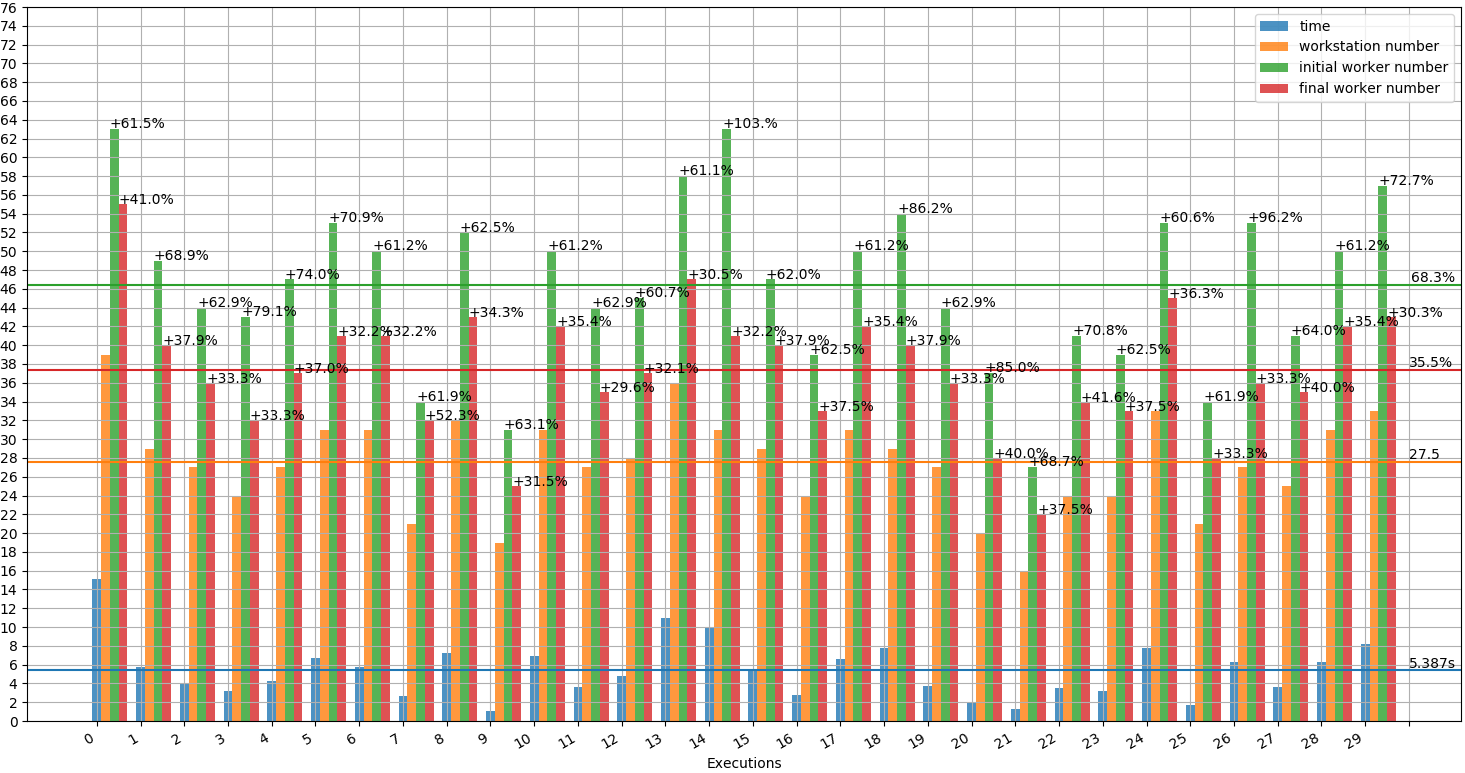
\includegraphics[width=21cm, keepaspectratio]{../immagini/executions.png}
        \caption{Grafico prodotto dai test: Executions}\label{fig67}
    \end{sidewaysfigure}
    \FloatBarrier
    \noindent 
    
    \paragraph{Grafici ``Tests''} Sono tre grafici diversi che mostrano l'attuazione del modello probabilistico negli input generati dal programma. \\
    \\ Il primo mostra la distribuzione dei livelli sulle postazioni e sui lavoratori. Ricordando che la distribuzione dei livelli sulle postazioni deve seguire la distribuzione discreta uniforme, mentre la distribuzione dei livelli sui lavoratori deve seguire la distribuzione normale (gaussiana), su trenta esecuzioni dell’algoritmo sono state prodotte le distribuzioni visibili in \hyperref[fig68]{Figura 6.8}, che confermano il modello probabilistico:
    \begin{figure}[!h]
        \label{fig68}
            \centering
            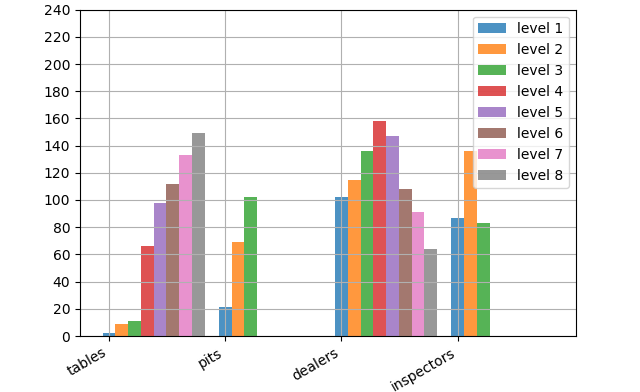
\includegraphics[width=0.8\textwidth,keepaspectratio]{../immagini/tests_levels.png}
            \caption{Grafico prodotto dai test: Tests (livelli)}
    \end{figure}
    \FloatBarrier
    \noindent
    Il secondo grafico mostra la distribuzione della conoscenza dei giochi sulle postazioni e sui lavoratori (limitandosi ai dealer, in quanto dealer-inspector e inspector conoscono tutti i giochi). Ricordando che la frequenza dei giochi deve essere il 50\% per il gioco base // e il 25\% per BJ e PG, su trenta esecuzioni dell’algoritmo sono state prodotte le distribuzioni visibili in \hyperref[fig69]{Figura 6.9}, che confermano il modello probabilistico:
    \begin{figure}[!h]
        \label{fig69}
            \centering
            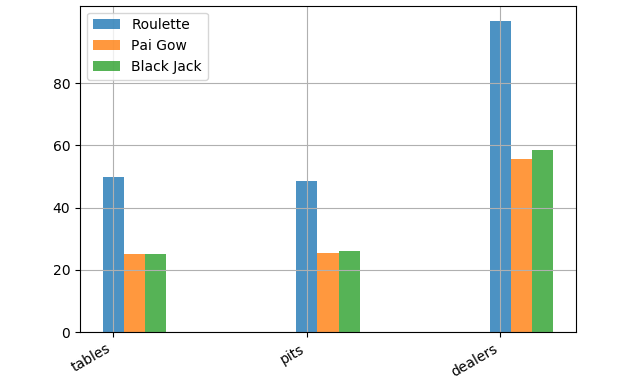
\includegraphics[width=0.8\textwidth,keepaspectratio]{../immagini/tests_games.png}
            \caption{Grafico prodotto dai test: Tests (giochi)}
    \end{figure}
    \FloatBarrier
    \noindent
    Il terzo e ultimo grafico mostra la distribuzione della conoscenza dei giochi sui dealer, suddivisi per livello. Ricordando che la probabilità che un dealer conosca un gioco è direttamente proporzionale al suo livello secondo una distribuzione di Bernoulli (quindi, un livello 1 ha probabilità del 90\% di conoscere un gioco, un livello 2 probabilità 80\%, e così via fino ad arrivare a un livello 8 che ha probabiblità del 20\%), su trenta esecuzioni dell’algoritmo sono state prodotte le distribuzioni visibili in \hyperref[fig610]{Figura 6.10}, che confermano il modello probabilistico:
    \begin{figure}[!h]
        \label{fig610}
        \centering
        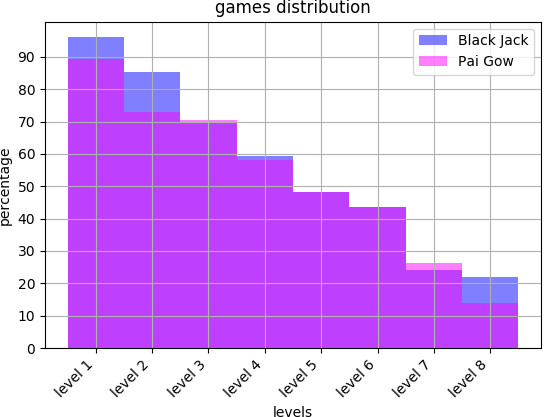
\includegraphics[width=0.8\textwidth,keepaspectratio]{../immagini/distr_games.png}
        \caption{Grafico prodotto dai test: Tests (giochi per livelli)}
    \end{figure}
    \FloatBarrier
    \noindent
    
    \paragraph{Grafici ``Exec n''} Infine per ogni esecuzione viene creato un grafico (quindi in tutto, per un'esecuzione dello script, vengono creati trenta grafici) per mostrare la bontà degli input prodotti; essi mostrano il numero di lavoratori prodotti dal modello probabilistico capaci di lavorare in ogni postazione e possono essere di due colori: rosso o verde.\\
    I grafici rossi indicano che i lavoratori prodotti come input per l'esecuzione \textit{n} non erano ben distribuiti sui tavoli; l'algoritmo non ha quindi trovato una soluzione ammissibile e ha dovuto inserire nello schedule il Dummy Worker. \\
    I grafici verdi, al contrario, indicano che l'algoritmo ha trovato una soluzione ammissibile.\\
    Assumendo che l'algoritmo greedy di riempimento dello scheduling funzioni correttamente, ovvero che trovi una soluzione ammissibile quando ce ne è una, tali grafici diventano una misura della bontà dell'input prodotta dal modello probabilistico.
    Nella \hyperref[fig611]{Figura 6.11} si possono vedere le due tipologie di grafici; si noti come nel grafico rosso a sinistra ci siano delle postazioni con un numero molto basso di lavoratori disponibili, mentre nel grafico verde a destra i lavoratori siano meglio distribuiti sulle postazioni.
    
    \begin{figure}[!h]
        \label{fig611}
        \begin{widepage}
            \centering
            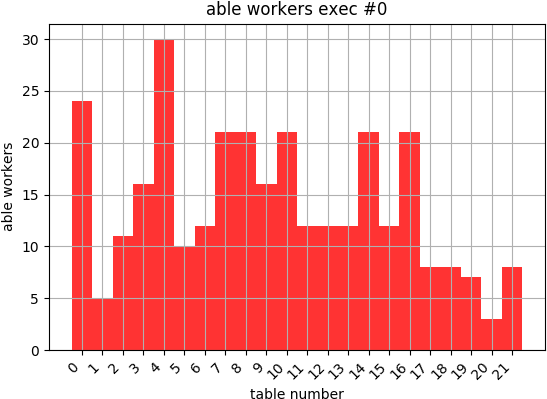
\includegraphics[width=.49\textwidth]{../immagini/exec_0.png}\hfil
            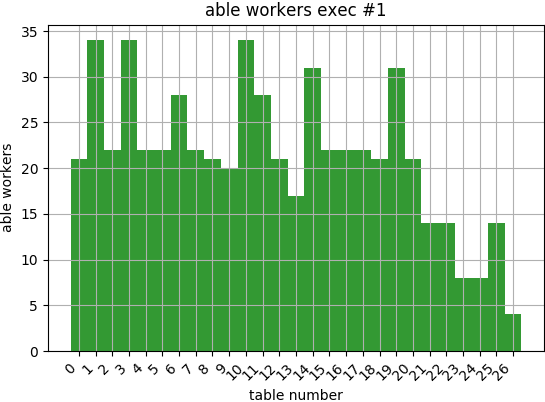
\includegraphics[width=.49\textwidth]{../immagini/exec_1.png}
            \caption{Grafici prodotti dai test: Exec n}
        \end{widepage}
    \end{figure}
    \FloatBarrier
    \noindent
   
   \subsection{Analisi dei risultati}
   Sono stati eseguiti tre test prestazionali modificando lievemente i parametri del modello di generazione degli input, al fine di provare a rispecchiare diversi tipi di situazioni che possono presentarsi all'interno del casinò e per analizzare le reazioni dell'algoritmo.
   \subsubsection{Primo test prestazionale}
   Il test viene eseguito sulla distribuzione uniforme dei livelli delle postazioni, tuttavia limitando ad un numero basso (tra 0 e un decimo del numero di tavoli) i livelli molto alti (sotto il tre) assegnati ai tavoli.\\
   Questa istanza di test è stata ripetuta tre volte per 30 esecuzioni ciascuna.\\
   I grafici sulle distribuzioni di giochi e livelli hanno confermato le premesse. Nella \hyperref[tab:test_1]{Tabella 6.1} vengono riassunti i risultati ottenuti.
       \begin{table}[!h]
           \caption{Risultati del primo test prestazionale}
           \label{tab:test_1}
           \begin{tabularx}{\textwidth}{|X|c|c|c|}
               \hline
               \thead{} & \thead{Test 1} & \thead{Test 2} & \thead{Test 3}\\
               \hline
               Presenza del dummy worker & 4 / 30 & 8 / 30 & 7 / 30 \\
               \hline
               Tempo di esecuzione medio & 3.410s & 3.662s	 & 4.526s \\
               \hline
               Percentuale di lavoratori iniziali &+58.9\%&+57.8\%&+60.2\% \\
               \hline
               Percentuale di lavoratori ottimizzati &+35.5\%&+34.3\%&+35.2\%
                \\
               \hline
           \end{tabularx}
       \end{table}%
    \FloatBarrier
    \noindent
    L'analisi delle soluzioni non ammissibili e degli input che le hanno generate hanno evidenziato che in un caso non era stata trovata una soluzione ammissibile a causa di una cattiva rotazione delle limitate risorse disponibili per coprire alcune postazioni; risolvendo il problema a mano, con un'oculata rotazione era possibile creare una soluzione ammissibile, compiendo però delle scelte che vanno contro la scelta greedy. Si riconosce il limite dell'euristica. \\
    Negli altri casi, le soluzioni non ammissibili sono dovute a un input iniziale non ben distribuito.
    
   \subsubsection{Secondo test prestazionale}
   Il test viene eseguito sulla seguente distribuzione dei livelli delle postazioni: i tavoli di livello alto (sotto il 3) sono limitati ad un numero basso (tra 0 e un decimo del numero dei tavoli); gli altri tavoli sono tutti di livello molto basso (8).\\
   Questa istanza di test è stata ripetuta tre volte per 30 esecuzioni ciascuna.\\
   I grafici sulle distribuzioni di giochi e livelli hanno confermato le premesse. Nella \hyperref[tab:test_2]{Tabella 6.2} vengono riassunti i risultati ottenuti.
   \begin{table}[!h]
       \caption{Risultati del secondo test prestazionale}
       \label{tab:test_2}
       \begin{tabularx}{\textwidth}{|X|c|c|c|}
           \hline
           \thead{} & \thead{Test 1} & \thead{Test 2} & \thead{Test 3}\\
           \hline
           Presenza del dummy worker & 5 / 30 & 6 / 30 & 7 / 30 \\
           \hline
           Tempo di esecuzione medio & 4.197s & 5.387s	 & 4.205s \\
           \hline
           Percentuale di lavoratori iniziali &+68.2\%&+68.3\%&+66.1\% \\
           \hline
           Percentuale di lavoratori ottimizzati &+35.6\%&+34.5\%&+36.3\%
           \\
           \hline
       \end{tabularx}
   \end{table}%
   \FloatBarrier
   \noindent
   L'analisi delle soluzioni non ammissibili non ha rivelato criticità, se non per un caso di seguito descritto, in quanto sono dovute a un input iniziale non ben distribuito.\\
   Tuttavia è stata osservata un'anomalia all'interno di una soluzione non ammissibile: due lavoratori che si alternano in modo anomalo su un tavolo rimanendo in pausa per moltissimi turni consecutivi. Ciò è dovuto al fatto che sono inspector di livello 1 e c'è solo un pit di livello 1. L'algoritmo preferisce mettere altri lavoratori meno qualificati nei pit di livello 2-3, perciò dopo che i due lavoratori in esame vanno in pausa vengono raramente assegnati ad un altro pit. Ciò preclude loro la possibilità di tornare a lavorare nell'unico pit di livello 1, perché dopo la pausa devono cambiare per forza postazione. A ciò è dovuto anche l'utilizzo del dummy worker. Si riconosce il limite dell'euristica. \\
    
   \subsubsection{Terzo test prestazionale}
   Il test viene eseguito sulla seguente distribuzione dei livelli delle postazioni: i tavoli di livello alto (sotto il 3) sono limitati ad un numero basso (tra 0 e un decimo del numero dei tavoli); gli altri tavoli sono tutti di livello molto basso (8). Inoltre tutti i pit sono di livello 3. Questa istanza di test è ritenuta la più importante perché rispetta al meglio la distribuzione dei tavoli all'interno del casinò di Londra.\\
   Questa istanza di test è stata ripetuta tre volte per 30 esecuzioni ciascuna. I grafici sulle distribuzioni di giochi e livelli hanno confermato le premesse. Nella \hyperref[tab:test_3]{Tabella 6.3} vengono riassunti i risultati ottenuti.
   \begin{table}[!h]
       \caption{Risultati del terzo test prestazionale}
       \label{tab:test_3}
       \begin{tabularx}{\textwidth}{|X|c|c|c|}
           \hline
           \thead{} & \thead{Test 1} & \thead{Test 2} & \thead{Test 3}\\
           \hline
           Presenza del dummy worker & 0 / 30 & 1 / 30 & 1 / 30 \\
           \hline
           Tempo di esecuzione medio & 6.043s & 5.541s	 & 5.307s \\
           \hline
           Percentuale di lavoratori iniziali &+71.0\%&+68.7\%&+68.7\% \\
           \hline
           Percentuale di lavoratori ottimizzati &+36.9\%&+37.9\%&+37.4\%
           \\
           \hline
       \end{tabularx}
   \end{table}%
 \FloatBarrier
\noindent
L'analisi delle soluzioni non ammissibili non ha rivelato criticità, in quanto sono dovute a un input iniziale non ben distribuito.
\subsection{Conclusioni}
L'analisi delle soluzioni (ammissibili e non) prodotte dall'algoritmo è stata, in conclusione, soddisfacente. \\
L'algoritmo rispetta sempre i vincoli imposti dal problema e crea delle soluzioni buone sotto i seguenti punti di vista:
\begin{enumerate}
    \item dopo che un lavoratore è stato in pausa, l'algoritmo prioritizza il suo rientro nello scheduling, evitando di lasciarlo in pausa per più turni consecutivi;
    \item i turni dei lavoratori sono solitamente di tre o quattro scaglioni consecutivi; trovare cinque scaglioni consecutivi è raro (con un numero di lavoratori congruo);
    \item quando un lavoratore è schedulato per un turno in un certo tavolo, viene schedulato per quel tavolo anche nei turni immediatamente successivi per limitarne gli eccessivi spostamenti;
    \item a pari disponibilità di due lavoratori per una postazione, viene sempre scelto il lavoratore con il livello più adatto a ricoprire la posizione.
\end{enumerate}
Nonostante siano stati individuati dei limiti per l'algoritmo, essi sono stati ritenuti accettabili. Bisogna infatti ricordare che si tratta di un algoritmo euristico volto a trovare uno scheduling iniziale ammissibile che faccia da base ad altri algoritmi metaeuristici, quindi non solo per sua natura non può certamente trovare la soluzione ottima, ma anche gli è concesso di compiere scelte greedy che a posteriori si rivelano, a volte, poco oculate. Sarà compito di una futura metaeuristica sopperire alle mancanze del corrente algoritmo greedy.